% 1977 年山东A卷第 2 题：三角形 ABC 的外接圆，AD 为高（D 在 BC 上），E 在 BC 上且 A、E、F 共线，F 为 AE 延长线与圆的交点，CF 为虚线辅助线（按源卷第 2 页布局）
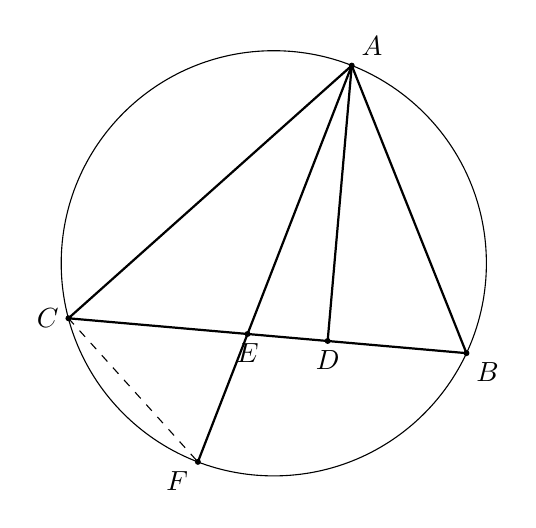
\begin{tikzpicture}[scale=0.9]
  \draw (0,0) circle (3);
  \coordinate (A) at (1.1,2.79);
  \coordinate (B) at (2.719,-1.268);
  \coordinate (C) at (-2.898,-0.776);
  \coordinate (D) at (0.760,-1.096);
  \coordinate (E) at (-0.370,-0.997);
  \coordinate (F) at (-1.071,-2.802);
  \draw[thick] (A) -- (B) -- (C) -- cycle;
  \draw[thick] (A) -- (D);
  \draw[thick] (A) -- (F);
  \draw[dashed] (C) -- (F);
  \fill (A) circle (1.2pt) node[above right] {$A$};
  \fill (B) circle (1.2pt) node[below right] {$B$};
  \fill (C) circle (1.2pt) node[left] {$C$};
  \fill (D) circle (1.2pt) node[below] {$D$};
  \fill (E) circle (1.2pt) node[below] {$E$};
  \fill (F) circle (1.2pt) node[below left] {$F$};
\end{tikzpicture}
